\section{Experimental results\label{section:results}}


% \begin{figure}[h!]
% \begin{center}
%  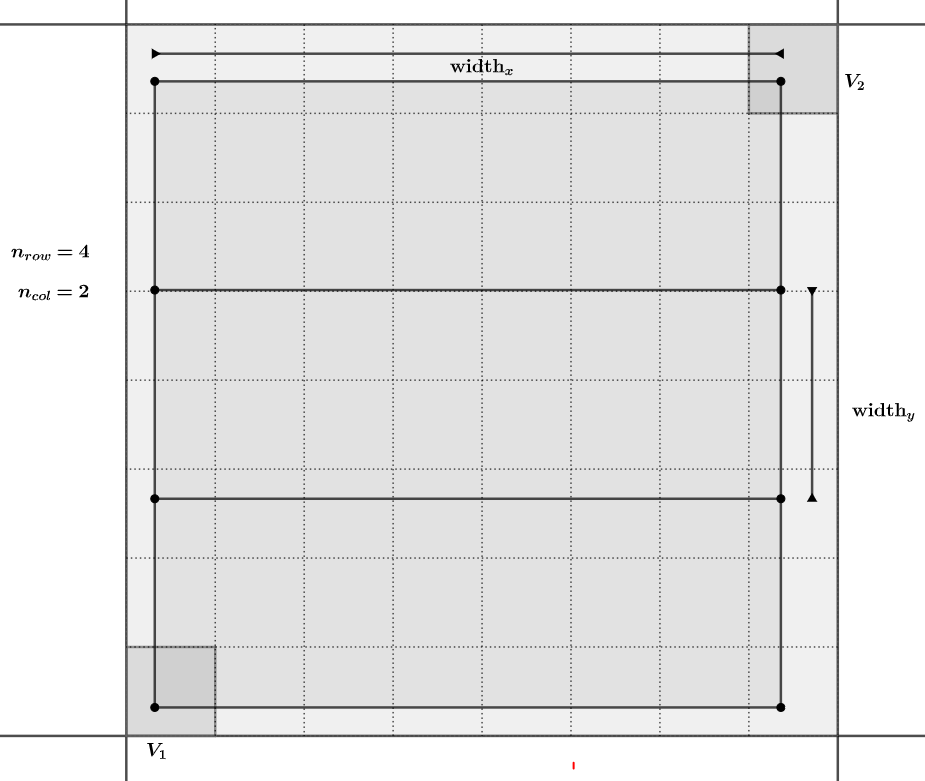
\includegraphics[width=1\linewidth]{Grid_generation.png}
% \end{center}
% \end{figure}
\noindent
In this section\RE{,} we discuss the experimental results obtained testing the formulations presented in Section \ref{Form} and the matheuristic procedure proposed in Section \ref{Math} on a testbed of instances. In particular, we consider instances like the ones used in \cite{art:Amorosi2021}\RE{,} where the targets to be visited by the drones are represented by grid graphs.
\RE{We have generated one set of 5 instances with 5 graphs and \RE{another} set of 5 instances with 10 graphs.} More precisely, each instance is composed of 20$\%$ graphs with 4 nodes, 20$\%$ graphs of 6 nodes, 20$\%$ graphs of 8 nodes, 20$\%$ graphs of 10 nodes and \RE{and 20$\%$ graphs with 12 nodes}. Moreover, we assume that the velocity of the drones is twice that of the mothership and that a random \RE{fraction} of each target graph, or of each of its edges, must be visited by the fleet of drones. \RE{These fractions are uniform randomly sampled in the interval $(0, 1)$.}\\

%\subsection{\CV{ADD TITLE TO THE FIRST EXPERIMENT}} 
We consider in our experiments that the number of drones varies between 1 and 3 and that the drone endurance (expressed as \RE{the} maximum time that the drone can operate when it is fully recharged) ranges between 20 and 60. \RE{Note that the case of a single drone is also included in our experiments to compare the results and complexity of using one and more than one drones. \RE{The interested reader is referred to \cite{art:Amorosi2021} for analyzing} the complexity in terms of gap of the model with a single drone.}
Table \ref{table:tab1} reports a summary of the characteristics of our instances.

\renewcommand{\arraystretch}{0.7}
\begin{table}[!h]
\caption{Instances parameter values}
\centering
\footnotesize
\begin{tabular}{c | c }
\hline
\RE{$|\mathcal G|$} & (5,10)\\
\hline
\RE{$|\mathcal D|$} &	(1,2,3)\\
\hline
\RE{$|V_g|$} & (4,6,8,10,12)\\
\hline
\RE{$N_D$} & (20,30,40,50,60)\\
\hline
\RE{fraction} target (edge) & \RE{uniform randomly sampled in $(0, 1)$.}
\end{tabular}
\label{table:tab1}
\end{table}

\noindent
Table \ref{table:tab2} reports the results obtained solving the \AMMDRPG model on the instances previously described, by adopting the commercial solver Gurobi. We consider the exact solution both providing and not providing an initial solution computed by the matheuristic described in Section \ref{Math}. More precisely, the first column of Table \ref{table:tab2} indicates the number of target graphs to be visited by the fleet of drones, the second column reports the \RE{endurance} of the drones, the third column distinguishes between the visit of a \RE{fraction} of each edge (e) and a \RE{fraction} of each target graph (g). The fourth column reports the size of the fleet of drones. \RE{This last column contains three subcolumns reporting, for each cardinality of the set $\mathcal D$, respectively, the average percentage gap with initialization by the solution provided by the matheuristic (i), the solution time, in seconds, of the matheuristic (TimeH) and the average percentage gap without initialization by the solution obtained by the matheuristic (wi) for each combination of the listed parameters. The time limit of these experiments is set equal to 2 hours.}\\

We can observe that the value of the average percentage gap ranges between a minimum of 66.9\% and a maximum of 97.43\%. This shows that the model is hard to be solved even with small size instances. Moreover, we can see that in most of the cases, the average percentage gap associated with the variant of the model consisting in visiting a given \RE{fraction} of each edge, is higher than the one associated with the variant imposing to visit a given \RE{fraction} of each target graph. Another thing that we can observe is that the average percentage gap increases with the number of drones and decreases with the drone endurance.\\
\noindent
As regards the number of target graphs, we can see that by increasing it from 5 to 10, the exact method without initialization \RE{of} the solution obtained with the \RE{matheuristic}, becomes even harder. Indeed, the red entries of the table mean that some instances could not find a feasible solution within the time limit (note that in the brackets we indicate the number of these instances). The number of not \RE{solved} instances increases with the number of drones. Moreover, for the minimum level of endurance, the exact solution of the model without initialization provided by the matheuristic, does not provide any solution within the time limit for instances with 10 graphs and 2 or 3 drones.\\
Considering the comparison with the exact method starting from the solution provided by the matheuristic, we can note that the values of the average percentage gap are very close to the ones related to the exact solution method without initialization. Thus\RE{,} the initialization does not speed up the convergence of the solver. However, we can see that the matheuristic is always able to find a feasible solution of the problem, even for the cases in which the solver is not. \RE{The boxplots in Figure \ref{fig:gap_boxplot_synchronous} represent the relative gap of the solution provided by the matheuristic with respect to the one provided by the exact solution of the \RE{mathematical programming} model within the time limit, with the initialization of the solution found by the matheuristic.}

% This file was created with tikzplotlib v0.9.12.
\definecolor{color0}{rgb}{0.917647058823529,0.917647058823529,0.949019607843137}
\definecolor{color1}{rgb}{0.347058823529412,0.458823529411765,0.641176470588235}
\definecolor{color2}{rgb}{0.798529411764706,0.536764705882353,0.389705882352941}

\begin{figure}[h!]
\centering
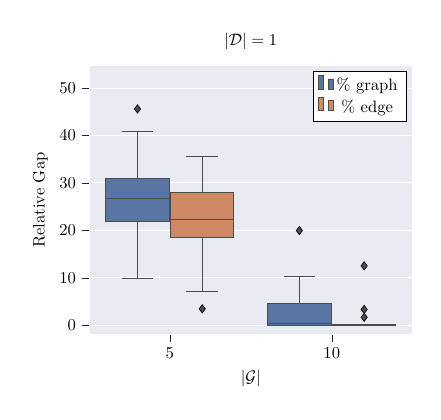
\begin{tikzpicture}[scale=0.6]

\begin{axis}[
axis background/.style={fill=color0},
axis line style={white},
tick align=outside,
title={$|\mathcal D| = 1$},
x grid style={white},
xtick pos = left,
ytick pos = left,
xlabel={$|\mathcal G|$},
xmin=-0.5, xmax=1.5,
xtick style={color=white!15!black},
xtick={0,1},
xticklabels={5,10},
y grid style={white},
ylabel={Relative Gap},
ymajorgrids,
ymin=-2.0023571013993, ymax=54.6854669223967,
ytick style={color=white!15!black}
]
\path [draw=white!29.8039215686275!black, fill=color1, semithick]
(axis cs:-0.396,21.7888049191559)
--(axis cs:-0.004,21.7888049191559)
--(axis cs:-0.004,30.8406843661928)
--(axis cs:-0.396,30.8406843661928)
--(axis cs:-0.396,21.7888049191559)
--cycle;
\path [draw=white!29.8039215686275!black, fill=color2, semithick]
(axis cs:0.004,18.4793987935756)
--(axis cs:0.396,18.4793987935756)
--(axis cs:0.396,27.9849884101838)
--(axis cs:0.004,27.9849884101838)
--(axis cs:0.004,18.4793987935756)
--cycle;
\path [draw=white!29.8039215686275!black, fill=color1, semithick]
(axis cs:0.604,0.00874895880390045)
--(axis cs:0.996,0.00874895880390045)
--(axis cs:0.996,4.51419914610234)
--(axis cs:0.604,4.51419914610234)
--(axis cs:0.604,0.00874895880390045)
--cycle;
\path [draw=white!29.8039215686275!black, fill=color2, semithick]
(axis cs:1.004,0.0020834572568334)
--(axis cs:1.396,0.0020834572568334)
--(axis cs:1.396,0.0669377251793516)
--(axis cs:1.004,0.0669377251793516)
--(axis cs:1.004,0.0020834572568334)
--cycle;
\draw[draw=white!29.8039215686275!black,fill=color1,line width=0.3pt] (axis cs:0,0) rectangle (axis cs:0,0);
\draw[draw=white!29.8039215686275!black,fill=color1,line width=0.3pt] (axis cs:0,0) rectangle (axis cs:0,0);
\addlegendimage{ybar,ybar legend,draw=white!29.8039215686275!black,fill=color1,line width=0.3pt}
\addlegendentry{\% graph}

\draw[draw=white!29.8039215686275!black,fill=color2,line width=0.3pt] (axis cs:0,0) rectangle (axis cs:0,0);
\addlegendimage{ybar,ybar legend,draw=white!29.8039215686275!black,fill=color2,line width=0.3pt}
\addlegendentry{\% edge}

\addplot [semithick, white!29.8039215686275!black]
table {%
-0.2 21.7888049191559
-0.2 9.87718961543874
};
\addplot [semithick, white!29.8039215686275!black]
table {%
-0.2 30.8406843661928
-0.2 40.828071376835
};
\addplot [semithick, white!29.8039215686275!black]
table {%
-0.298 9.87718961543874
-0.102 9.87718961543874
};
\addplot [semithick, white!29.8039215686275!black]
table {%
-0.298 40.828071376835
-0.102 40.828071376835
};
\addplot [black, mark=diamond*, mark size=2.5, mark options={solid,fill=white!29.8039215686275!black}, only marks]
table {%
-0.2 45.5638022037681
};
\addplot [semithick, white!29.8039215686275!black]
table {%
0.2 18.4793987935756
0.2 7.03956951402302
};
\addplot [semithick, white!29.8039215686275!black]
table {%
0.2 27.9849884101838
0.2 35.4418303987987
};
\addplot [semithick, white!29.8039215686275!black]
table {%
0.102 7.03956951402302
0.298 7.03956951402302
};
\addplot [semithick, white!29.8039215686275!black]
table {%
0.102 35.4418303987987
0.298 35.4418303987987
};
\addplot [black, mark=diamond*, mark size=2.5, mark options={solid,fill=white!29.8039215686275!black}, only marks]
table {%
0.2 3.42933486135715
};
\addplot [semithick, white!29.8039215686275!black]
table {%
0.8 0.00874895880390045
0.8 0
};
\addplot [semithick, white!29.8039215686275!black]
table {%
0.8 4.51419914610234
0.8 10.2651385218831
};
\addplot [semithick, white!29.8039215686275!black]
table {%
0.702 0
0.898 0
};
\addplot [semithick, white!29.8039215686275!black]
table {%
0.702 10.2651385218831
0.898 10.2651385218831
};
\addplot [black, mark=diamond*, mark size=2.5, mark options={solid,fill=white!29.8039215686275!black}, only marks]
table {%
0.8 19.9251319119723
};
\addplot [semithick, white!29.8039215686275!black]
table {%
1.2 0.0020834572568334
1.2 -1.3353502544535e-14
};
\addplot [semithick, white!29.8039215686275!black]
table {%
1.2 0.0669377251793516
1.2 0.0939379065004709
};
\addplot [semithick, white!29.8039215686275!black]
table {%
1.102 -1.3353502544535e-14
1.298 -1.3353502544535e-14
};
\addplot [semithick, white!29.8039215686275!black]
table {%
1.102 0.0939379065004709
1.298 0.0939379065004709
};
\addplot [black, mark=diamond*, mark size=2.5, mark options={solid,fill=white!29.8039215686275!black}, only marks]
table {%
1.2 3.30798611427499
1.2 1.65360546285996
1.2 12.4879588505733
};
\addplot [semithick, white!29.8039215686275!black]
table {%
-0.396 26.6321353435948
-0.004 26.6321353435948
};
\addplot [semithick, white!29.8039215686275!black]
table {%
0.004 22.3311968283402
0.396 22.3311968283402
};
\addplot [semithick, white!29.8039215686275!black]
table {%
0.604 0.241511938215122
0.996 0.241511938215122
};
\addplot [semithick, white!29.8039215686275!black]
table {%
1.004 0.0136998158227596
1.396 0.0136998158227596
};
\end{axis}
\end{tikzpicture}
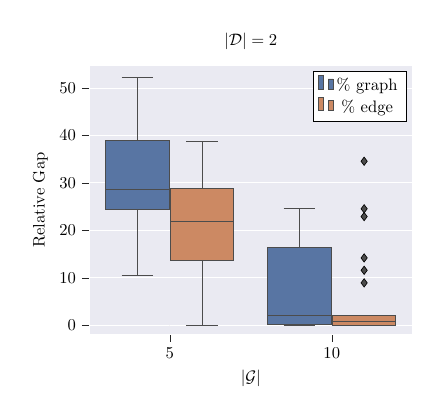
\begin{tikzpicture}[scale = 0.6]
\begin{axis}[
axis background/.style={fill=color0},
axis line style={white},
tick align=outside,
title={$|\mathcal D| = 2$},
x grid style={white},
xtick pos = left,
ytick pos = left,
xlabel={$|\mathcal G|$},
xmin=-0.5, xmax=1.5,
xtick style={color=white!15!black},
xtick={0,1},
xticklabels={5,10},
y grid style={white},
ylabel={Relative Gap},
ymajorgrids,
ymin=-2.0023571013993, ymax=54.6854669223967,
ytick style={color=white!15!black}
]
\path [draw=white!29.8039215686275!black, fill=color1, semithick]
(axis cs:-0.396,24.2908680304667)
--(axis cs:-0.004,24.2908680304667)
--(axis cs:-0.004,38.9734345321689)
--(axis cs:-0.396,38.9734345321689)
--(axis cs:-0.396,24.2908680304667)
--cycle;
\path [draw=white!29.8039215686275!black, fill=color2, semithick]
(axis cs:0.004,13.6199008648404)
--(axis cs:0.396,13.6199008648404)
--(axis cs:0.396,28.8801759071672)
--(axis cs:0.004,28.8801759071672)
--(axis cs:0.004,13.6199008648404)
--cycle;
\path [draw=white!29.8039215686275!black, fill=color1, semithick]
(axis cs:0.604,0.0328401107308227)
--(axis cs:0.996,0.0328401107308227)
--(axis cs:0.996,16.3389014643552)
--(axis cs:0.604,16.3389014643552)
--(axis cs:0.604,0.0328401107308227)
--cycle;
\path [draw=white!29.8039215686275!black, fill=color2, semithick]
(axis cs:1.004,0.018119712131219)
--(axis cs:1.396,0.018119712131219)
--(axis cs:1.396,2.05799457575158)
--(axis cs:1.004,2.05799457575158)
--(axis cs:1.004,0.018119712131219)
--cycle;
\draw[draw=white!29.8039215686275!black,fill=color1,line width=0.3pt] (axis cs:0,0) rectangle (axis cs:0,0);
\addlegendimage{ybar,ybar legend,draw=white!29.8039215686275!black,fill=color1,line width=0.3pt}
\addlegendentry{\% graph}

\draw[draw=white!29.8039215686275!black,fill=color2,line width=0.3pt] (axis cs:0,0) rectangle (axis cs:0,0);
\addlegendimage{ybar,ybar legend,draw=white!29.8039215686275!black,fill=color2,line width=0.3pt}
\addlegendentry{\% edge}
\draw[draw=white!29.8039215686275!black,fill=color1,line width=0.3pt] (axis cs:0,0) rectangle (axis cs:0,0);
\draw[draw=white!29.8039215686275!black,fill=color2,line width=0.3pt] (axis cs:0,0) rectangle (axis cs:0,0);
\addplot [semithick, white!29.8039215686275!black]
table {%
-0.2 24.2908680304667
-0.2 10.4474623283978
};
\addplot [semithick, white!29.8039215686275!black]
table {%
-0.2 38.9734345321689
-0.2 52.0813970689492
};
\addplot [semithick, white!29.8039215686275!black]
table {%
-0.298 10.4474623283978
-0.102 10.4474623283978
};
\addplot [semithick, white!29.8039215686275!black]
table {%
-0.298 52.0813970689492
-0.102 52.0813970689492
};
\addplot [semithick, white!29.8039215686275!black]
table {%
0.2 13.6199008648404
0.2 7.13365300294341e-06
};
\addplot [semithick, white!29.8039215686275!black]
table {%
0.2 28.8801759071672
0.2 38.6874614170675
};
\addplot [semithick, white!29.8039215686275!black]
table {%
0.102 7.13365300294341e-06
0.298 7.13365300294341e-06
};
\addplot [semithick, white!29.8039215686275!black]
table {%
0.102 38.6874614170675
0.298 38.6874614170675
};
\addplot [semithick, white!29.8039215686275!black]
table {%
0.8 0.0328401107308227
0.8 0
};
\addplot [semithick, white!29.8039215686275!black]
table {%
0.8 16.3389014643552
0.8 24.5633566326984
};
\addplot [semithick, white!29.8039215686275!black]
table {%
0.702 0
0.898 0
};
\addplot [semithick, white!29.8039215686275!black]
table {%
0.702 24.5633566326984
0.898 24.5633566326984
};
\addplot [semithick, white!29.8039215686275!black]
table {%
1.2 0.018119712131219
1.2 0
};
\addplot [semithick, white!29.8039215686275!black]
table {%
1.2 2.05799457575158
1.2 2.05799457575158
};
\addplot [semithick, white!29.8039215686275!black]
table {%
1.102 0
1.298 0
};
\addplot [semithick, white!29.8039215686275!black]
table {%
1.102 2.05799457575158
1.298 2.05799457575158
};
\addplot [black, mark=diamond*, mark size=2.5, mark options={solid,fill=white!29.8039215686275!black}, only marks]
table {%
1.2 11.5527375588776
1.2 22.8746077530694
1.2 24.5217334511995
1.2 34.5349113191651
1.2 8.9029594424669
1.2 14.1613847472345
};
\addplot [semithick, white!29.8039215686275!black]
table {%
-0.396 28.4878031388385
-0.004 28.4878031388385
};
\addplot [semithick, white!29.8039215686275!black]
table {%
0.004 21.8875260151041
0.396 21.8875260151041
};
\addplot [semithick, white!29.8039215686275!black]
table {%
0.604 1.99685736233386
0.996 1.99685736233386
};
\addplot [semithick, white!29.8039215686275!black]
table {%
1.004 0.672152105031548
1.396 0.672152105031548
};
\end{axis}
\end{tikzpicture}
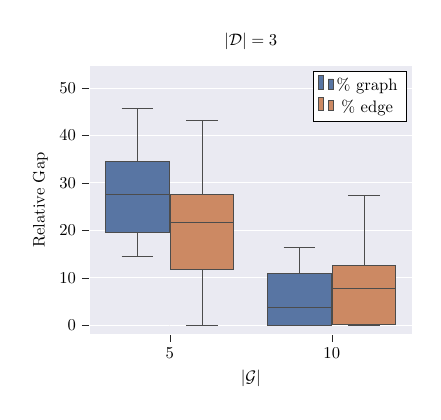
\begin{tikzpicture}[scale = 0.6]
\begin{axis}[
axis background/.style={fill=color0},
axis line style={white},
tick align=outside,
title={$|\mathcal D| = 3$},
x grid style={white},
xtick pos = left,
ytick pos = left,
xlabel={$|\mathcal G|$},
xmin=-0.5, xmax=1.5,
xtick style={color=white!15!black},
xtick={0,1},
xticklabels={5,10},
y grid style={white},
ylabel={Relative Gap},
ymajorgrids,
ymin=-2.0023571013993, ymax=54.6854669223967,
ytick style={color=white!15!black}
]
\path [draw=white!29.8039215686275!black, fill=color1, semithick]
(axis cs:-0.396,19.4786101400453)
--(axis cs:-0.004,19.4786101400453)
--(axis cs:-0.004,34.4617472367364)
--(axis cs:-0.396,34.4617472367364)
--(axis cs:-0.396,19.4786101400453)
--cycle;
\path [draw=white!29.8039215686275!black, fill=color2, semithick]
(axis cs:0.004,11.6307680369222)
--(axis cs:0.396,11.6307680369222)
--(axis cs:0.396,27.593386872566)
--(axis cs:0.004,27.593386872566)
--(axis cs:0.004,11.6307680369222)
--cycle;
\path [draw=white!29.8039215686275!black, fill=color1, semithick]
(axis cs:0.604,0.0153042661953022)
--(axis cs:0.996,0.0153042661953022)
--(axis cs:0.996,10.8860101762497)
--(axis cs:0.604,10.8860101762497)
--(axis cs:0.604,0.0153042661953022)
--cycle;
\path [draw=white!29.8039215686275!black, fill=color2, semithick]
(axis cs:1.004,0.0926366637998731)
--(axis cs:1.396,0.0926366637998731)
--(axis cs:1.396,12.6414099793463)
--(axis cs:1.004,12.6414099793463)
--(axis cs:1.004,0.0926366637998731)
--cycle;
\draw[draw=white!29.8039215686275!black,fill=color1,line width=0.3pt] (axis cs:0,0) rectangle (axis cs:0,0);
\addlegendimage{ybar,ybar legend,draw=white!29.8039215686275!black,fill=color1,line width=0.3pt}
\addlegendentry{\% graph}

\draw[draw=white!29.8039215686275!black,fill=color2,line width=0.3pt] (axis cs:0,0) rectangle (axis cs:0,0);
\addlegendimage{ybar,ybar legend,draw=white!29.8039215686275!black,fill=color2,line width=0.3pt}
\addlegendentry{\% edge}
\draw[draw=white!29.8039215686275!black,fill=color1,line width=0.3pt] (axis cs:0,0) rectangle (axis cs:0,0);
\draw[draw=white!29.8039215686275!black,fill=color2,line width=0.3pt] (axis cs:0,0) rectangle (axis cs:0,0);
\addplot [semithick, white!29.8039215686275!black]
table {%
-0.2 19.4786101400453
-0.2 14.3600714974331
};
\addplot [semithick, white!29.8039215686275!black]
table {%
-0.2 34.4617472367364
-0.2 45.5815915247392
};
\addplot [semithick, white!29.8039215686275!black]
table {%
-0.298 14.3600714974331
-0.102 14.3600714974331
};
\addplot [semithick, white!29.8039215686275!black]
table {%
-0.298 45.5815915247392
-0.102 45.5815915247392
};
\addplot [semithick, white!29.8039215686275!black]
table {%
0.2 11.6307680369222
0.2 0
};
\addplot [semithick, white!29.8039215686275!black]
table {%
0.2 27.593386872566
0.2 43.0903230193938
};
\addplot [semithick, white!29.8039215686275!black]
table {%
0.102 0
0.298 0
};
\addplot [semithick, white!29.8039215686275!black]
table {%
0.102 43.0903230193938
0.298 43.0903230193938
};
\addplot [semithick, white!29.8039215686275!black]
table {%
0.8 0.0153042661953022
0.8 0
};
\addplot [semithick, white!29.8039215686275!black]
table {%
0.8 10.8860101762497
0.8 16.4617414417269
};
\addplot [semithick, white!29.8039215686275!black]
table {%
0.702 0
0.898 0
};
\addplot [semithick, white!29.8039215686275!black]
table {%
0.702 16.4617414417269
0.898 16.4617414417269
};
\addplot [semithick, white!29.8039215686275!black]
table {%
1.2 0.0926366637998731
1.2 0
};
\addplot [semithick, white!29.8039215686275!black]
table {%
1.2 12.6414099793463
1.2 27.2419248135531
};
\addplot [semithick, white!29.8039215686275!black]
table {%
1.102 0
1.298 0
};
\addplot [semithick, white!29.8039215686275!black]
table {%
1.102 27.2419248135531
1.298 27.2419248135531
};
\addplot [semithick, white!29.8039215686275!black]
table {%
-0.396 27.5658718997128
-0.004 27.5658718997128
};
\addplot [semithick, white!29.8039215686275!black]
table {%
0.004 21.5787147317098
0.396 21.5787147317098
};
\addplot [semithick, white!29.8039215686275!black]
table {%
0.604 3.74263341643573
0.996 3.74263341643573
};
\addplot [semithick, white!29.8039215686275!black]
table {%
1.004 7.62592534857705
1.396 7.62592534857705
};
\end{axis}
\end{tikzpicture}
\caption{Relative gap boxplots for \AMDCO}
\label{fig:gap_boxplot_synchronous}
\end{figure}
% This file was created with tikzplotlib v0.9.16.
\begin{tikzpicture}

\definecolor{color0}{rgb}{0.917647058823529,0.917647058823529,0.949019607843137}
\definecolor{color1}{rgb}{0.347058823529412,0.458823529411765,0.641176470588235}
\definecolor{color2}{rgb}{0.798529411764706,0.536764705882353,0.389705882352941}

\begin{groupplot}[group style={group size=3 by 1}]
\nextgroupplot[
axis background/.style={fill=color0},
axis line style={white},
tick align=outside,
title={Num\_Drones = 1},
x grid style={white},
xlabel=\textcolor{white!15!black}{Size},
xmajorticks=false,
xmin=-0.5, xmax=1.5,
xtick style={color=white!15!black},
xtick={0,1},
xticklabels={5,10},
y grid style={white},
ylabel=\textcolor{white!15!black}{Difference},
ymajorgrids,
ymajorticks=false,
ymin=-2.63274851310481, ymax=55.287718775201,
ytick style={color=white!15!black}
]
\path [draw=white!29.8039215686275!black, fill=color1, semithick]
(axis cs:-0.396,28.3309607578556)
--(axis cs:-0.004,28.3309607578556)
--(axis cs:-0.004,38.3836190274944)
--(axis cs:-0.396,38.3836190274944)
--(axis cs:-0.396,28.3309607578556)
--cycle;
\path [draw=white!29.8039215686275!black, fill=color2, semithick]
(axis cs:0.004,0)
--(axis cs:0.396,0)
--(axis cs:0.396,8.64232854240097)
--(axis cs:0.004,8.64232854240097)
--(axis cs:0.004,0)
--cycle;
\path [draw=white!29.8039215686275!black, fill=color1, semithick]
(axis cs:0.604,20.1606294075813)
--(axis cs:0.996,20.1606294075813)
--(axis cs:0.996,32.0444971852192)
--(axis cs:0.604,32.0444971852192)
--(axis cs:0.604,20.1606294075813)
--cycle;
\path [draw=white!29.8039215686275!black, fill=color2, semithick]
(axis cs:1.004,0)
--(axis cs:1.396,0)
--(axis cs:1.396,0)
--(axis cs:1.004,0)
--(axis cs:1.004,0)
--cycle;
\draw[draw=white!29.8039215686275!black,fill=color1,line width=0.3pt] (axis cs:0,0) rectangle (axis cs:0,0);
\addlegendimage{ybar,ybar legend,draw=white!29.8039215686275!black,fill=color1,line width=0.3pt}
\addlegendentry{False}

\draw[draw=white!29.8039215686275!black,fill=color2,line width=0.3pt] (axis cs:0,0) rectangle (axis cs:0,0);
\addlegendimage{ybar,ybar legend,draw=white!29.8039215686275!black,fill=color2,line width=0.3pt}
\addlegendentry{True}

\addplot [semithick, white!29.8039215686275!black]
table {%
-0.2 28.3309607578556
-0.2 19.9489819152654
};
\addplot [semithick, white!29.8039215686275!black]
table {%
-0.2 38.3836190274944
-0.2 46.7554203427056
};
\addplot [semithick, white!29.8039215686275!black]
table {%
-0.298 19.9489819152654
-0.102 19.9489819152654
};
\addplot [semithick, white!29.8039215686275!black]
table {%
-0.298 46.7554203427056
-0.102 46.7554203427056
};
\addplot [semithick, white!29.8039215686275!black]
table {%
0.2 0
0.2 0
};
\addplot [semithick, white!29.8039215686275!black]
table {%
0.2 8.64232854240097
0.2 19.3163569560286
};
\addplot [semithick, white!29.8039215686275!black]
table {%
0.102 0
0.298 0
};
\addplot [semithick, white!29.8039215686275!black]
table {%
0.102 19.3163569560286
0.298 19.3163569560286
};
\addplot [semithick, white!29.8039215686275!black]
table {%
0.8 20.1606294075813
0.8 8.61694572924211
};
\addplot [semithick, white!29.8039215686275!black]
table {%
0.8 32.0444971852192
0.8 44.9150868750959
};
\addplot [semithick, white!29.8039215686275!black]
table {%
0.702 8.61694572924211
0.898 8.61694572924211
};
\addplot [semithick, white!29.8039215686275!black]
table {%
0.702 44.9150868750959
0.898 44.9150868750959
};
\addplot [semithick, white!29.8039215686275!black]
table {%
1.2 0
1.2 0
};
\addplot [semithick, white!29.8039215686275!black]
table {%
1.2 0
1.2 0
};
\addplot [semithick, white!29.8039215686275!black]
table {%
1.102 0
1.298 0
};
\addplot [semithick, white!29.8039215686275!black]
table {%
1.102 0
1.298 0
};
\addplot [black, mark=diamond*, mark size=2.5, mark options={solid,fill=white!29.8039215686275!black}, only marks]
table {%
1.2 12.5888829044052
1.2 3.60848275911591
1.2 12.6583395502889
1.2 13.9716744025076
1.2 16.3270267089377
};
\addplot [semithick, white!29.8039215686275!black]
table {%
-0.396 30.9387019139685
-0.004 30.9387019139685
};
\addplot [semithick, white!29.8039215686275!black]
table {%
0.004 0
0.396 0
};
\addplot [semithick, white!29.8039215686275!black]
table {%
0.604 28.5798952809469
0.996 28.5798952809469
};
\addplot [semithick, white!29.8039215686275!black]
table {%
1.004 0
1.396 0
};

\nextgroupplot[
axis background/.style={fill=color0},
axis line style={white},
scaled y ticks=manual:{}{\pgfmathparse{#1}},
tick align=outside,
title={Num\_Drones = 2},
x grid style={white},
xlabel=\textcolor{white!15!black}{Size},
xmajorticks=false,
xmin=-0.5, xmax=1.5,
xtick style={color=white!15!black},
xtick={0,1},
xticklabels={5,10},
y grid style={white},
ymajorgrids,
ymajorticks=false,
ymin=-2.63274851310481, ymax=55.287718775201,
ytick style={color=white!15!black},
yticklabels={}
]
\path [draw=white!29.8039215686275!black, fill=color1, semithick]
(axis cs:-0.396,28.9528671388206)
--(axis cs:-0.004,28.9528671388206)
--(axis cs:-0.004,39.4527135830959)
--(axis cs:-0.396,39.4527135830959)
--(axis cs:-0.396,28.9528671388206)
--cycle;
\path [draw=white!29.8039215686275!black, fill=color2, semithick]
(axis cs:0.004,0)
--(axis cs:0.396,0)
--(axis cs:0.396,9.17745409922012)
--(axis cs:0.004,9.17745409922012)
--(axis cs:0.004,0)
--cycle;
\path [draw=white!29.8039215686275!black, fill=color1, semithick]
(axis cs:0.604,8.28029279866768)
--(axis cs:0.996,8.28029279866768)
--(axis cs:0.996,27.2510559932073)
--(axis cs:0.604,27.2510559932073)
--(axis cs:0.604,8.28029279866768)
--cycle;
\path [draw=white!29.8039215686275!black, fill=color2, semithick]
(axis cs:1.004,0)
--(axis cs:1.396,0)
--(axis cs:1.396,0.474550632215708)
--(axis cs:1.004,0.474550632215708)
--(axis cs:1.004,0)
--cycle;
\draw[draw=white!29.8039215686275!black,fill=color1,line width=0.3pt] (axis cs:0,0) rectangle (axis cs:0,0);
\draw[draw=white!29.8039215686275!black,fill=color2,line width=0.3pt] (axis cs:0,0) rectangle (axis cs:0,0);
\addplot [semithick, white!29.8039215686275!black]
table {%
-0.2 28.9528671388206
-0.2 21.2691640675831
};
\addplot [semithick, white!29.8039215686275!black]
table {%
-0.2 39.4527135830959
-0.2 46.9606181956668
};
\addplot [semithick, white!29.8039215686275!black]
table {%
-0.298 21.2691640675831
-0.102 21.2691640675831
};
\addplot [semithick, white!29.8039215686275!black]
table {%
-0.298 46.9606181956668
-0.102 46.9606181956668
};
\addplot [semithick, white!29.8039215686275!black]
table {%
0.2 0
0.2 0
};
\addplot [semithick, white!29.8039215686275!black]
table {%
0.2 9.17745409922012
0.2 17.5208470985773
};
\addplot [semithick, white!29.8039215686275!black]
table {%
0.102 0
0.298 0
};
\addplot [semithick, white!29.8039215686275!black]
table {%
0.102 17.5208470985773
0.298 17.5208470985773
};
\addplot [semithick, white!29.8039215686275!black]
table {%
0.8 8.28029279866768
0.8 0
};
\addplot [semithick, white!29.8039215686275!black]
table {%
0.8 27.2510559932073
0.8 32.913522916207
};
\addplot [semithick, white!29.8039215686275!black]
table {%
0.702 0
0.898 0
};
\addplot [semithick, white!29.8039215686275!black]
table {%
0.702 32.913522916207
0.898 32.913522916207
};
\addplot [semithick, white!29.8039215686275!black]
table {%
1.2 0
1.2 0
};
\addplot [semithick, white!29.8039215686275!black]
table {%
1.2 0.474550632215708
1.2 0.474550632215708
};
\addplot [semithick, white!29.8039215686275!black]
table {%
1.102 0
1.298 0
};
\addplot [semithick, white!29.8039215686275!black]
table {%
1.102 0.474550632215708
1.298 0.474550632215708
};
\addplot [black, mark=diamond*, mark size=2.5, mark options={solid,fill=white!29.8039215686275!black}, only marks]
table {%
1.2 12.1727362614165
1.2 3.41452646013145
1.2 4.47475120605025
1.2 1.75525190654208
1.2 20.0853334870759
1.2 5.71472509020636
};
\addplot [semithick, white!29.8039215686275!black]
table {%
-0.396 33.9902877215194
-0.004 33.9902877215194
};
\addplot [semithick, white!29.8039215686275!black]
table {%
0.004 2.5545714022041
0.396 2.5545714022041
};
\addplot [semithick, white!29.8039215686275!black]
table {%
0.604 20.1286256305174
0.996 20.1286256305174
};
\addplot [semithick, white!29.8039215686275!black]
table {%
1.004 0
1.396 0
};

\nextgroupplot[
axis background/.style={fill=color0},
axis line style={white},
scaled y ticks=manual:{}{\pgfmathparse{#1}},
tick align=outside,
title={Num\_Drones = 3},
x grid style={white},
xlabel=\textcolor{white!15!black}{Size},
xmajorticks=false,
xmin=-0.5, xmax=1.5,
xtick style={color=white!15!black},
xtick={0,1},
xticklabels={5,10},
y grid style={white},
ymajorgrids,
ymajorticks=false,
ymin=-2.63274851310481, ymax=55.287718775201,
ytick style={color=white!15!black},
yticklabels={}
]
\path [draw=white!29.8039215686275!black, fill=color1, semithick]
(axis cs:-0.396,20.6502328956822)
--(axis cs:-0.004,20.6502328956822)
--(axis cs:-0.004,42.0703378382816)
--(axis cs:-0.396,42.0703378382816)
--(axis cs:-0.396,20.6502328956822)
--cycle;
\path [draw=white!29.8039215686275!black, fill=color2, semithick]
(axis cs:0.004,0)
--(axis cs:0.396,0)
--(axis cs:0.396,4.26271965023279)
--(axis cs:0.004,4.26271965023279)
--(axis cs:0.004,0)
--cycle;
\path [draw=white!29.8039215686275!black, fill=color1, semithick]
(axis cs:0.604,6.51356157805267)
--(axis cs:0.996,6.51356157805267)
--(axis cs:0.996,20.2474952370876)
--(axis cs:0.604,20.2474952370876)
--(axis cs:0.604,6.51356157805267)
--cycle;
\path [draw=white!29.8039215686275!black, fill=color2, semithick]
(axis cs:1.004,0)
--(axis cs:1.396,0)
--(axis cs:1.396,0.555979912554276)
--(axis cs:1.004,0.555979912554276)
--(axis cs:1.004,0)
--cycle;
\draw[draw=white!29.8039215686275!black,fill=color1,line width=0.3pt] (axis cs:0,0) rectangle (axis cs:0,0);
\draw[draw=white!29.8039215686275!black,fill=color2,line width=0.3pt] (axis cs:0,0) rectangle (axis cs:0,0);
\addplot [semithick, white!29.8039215686275!black]
table {%
-0.2 20.6502328956822
-0.2 10.2471902296757
};
\addplot [semithick, white!29.8039215686275!black]
table {%
-0.2 42.0703378382816
-0.2 52.6549702620961
};
\addplot [semithick, white!29.8039215686275!black]
table {%
-0.298 10.2471902296757
-0.102 10.2471902296757
};
\addplot [semithick, white!29.8039215686275!black]
table {%
-0.298 52.6549702620961
-0.102 52.6549702620961
};
\addplot [semithick, white!29.8039215686275!black]
table {%
0.2 0
0.2 0
};
\addplot [semithick, white!29.8039215686275!black]
table {%
0.2 4.26271965023279
0.2 6.73555632363422
};
\addplot [semithick, white!29.8039215686275!black]
table {%
0.102 0
0.298 0
};
\addplot [semithick, white!29.8039215686275!black]
table {%
0.102 6.73555632363422
0.298 6.73555632363422
};
\addplot [black, mark=diamond*, mark size=2.5, mark options={solid,fill=white!29.8039215686275!black}, only marks]
table {%
0.2 11.226703479259
0.2 18.440540898481
};
\addplot [semithick, white!29.8039215686275!black]
table {%
0.8 6.51356157805267
0.8 0
};
\addplot [semithick, white!29.8039215686275!black]
table {%
0.8 20.2474952370876
0.8 38.7549619542079
};
\addplot [semithick, white!29.8039215686275!black]
table {%
0.702 0
0.898 0
};
\addplot [semithick, white!29.8039215686275!black]
table {%
0.702 38.7549619542079
0.898 38.7549619542079
};
\addplot [black, mark=diamond*, mark size=2.5, mark options={solid,fill=white!29.8039215686275!black}, only marks]
table {%
0.8 42.3378604573217
};
\addplot [semithick, white!29.8039215686275!black]
table {%
1.2 0
1.2 0
};
\addplot [semithick, white!29.8039215686275!black]
table {%
1.2 0.555979912554276
1.2 1.02560932509559
};
\addplot [semithick, white!29.8039215686275!black]
table {%
1.102 0
1.298 0
};
\addplot [semithick, white!29.8039215686275!black]
table {%
1.102 1.02560932509559
1.298 1.02560932509559
};
\addplot [black, mark=diamond*, mark size=2.5, mark options={solid,fill=white!29.8039215686275!black}, only marks]
table {%
1.2 5.74957300316297
1.2 6.83050314587957
1.2 3.05802944269869
1.2 3.2945915803322
1.2 7.10699033092534
};
\addplot [semithick, white!29.8039215686275!black]
table {%
-0.396 33.1423283804038
-0.004 33.1423283804038
};
\addplot [semithick, white!29.8039215686275!black]
table {%
0.004 0
0.396 0
};
\addplot [semithick, white!29.8039215686275!black]
table {%
0.604 11.9971737488885
0.996 11.9971737488885
};
\addplot [semithick, white!29.8039215686275!black]
table {%
1.004 0
1.396 0
};
\end{groupplot}

\end{tikzpicture}


\RE{INCLUDE EXPLANATION OF THE BOXPLOTS}

Moreover, the average solution times of the matheuristic range between a minimum of 37 seconds to a maximum of 3 minutes. They increase with the drone \RE{endurance} for the variant of the model in which a given \RE{fraction} of each edge must be visited, while they decrease by increasing the number of drones for the variant of the model in which a given \RE{fraction} of each target graph must \RE{be} visited. By increasing the number of target graphs from 5 to 10, the average solution times of the matheuristic become more than double for both model variants.
Summing up, the results obtained show that the exact solution method given by solving the formulation is very challenging even for small size instances. However, exploiting it, the matheuristic is able to provide  solutions for all instances rather quickly.
% Please add the following required packages to your document preamble:
% Table generated by Excel2LaTeX from sheet 'Hoja2'
\begin{table}[htbp]
  \centering
  \caption{Add caption}
    \resizebox{\textwidth}{!}{
    \begin{tabular}{|c|c|c|ccc|ccc|ccc|ccc|}
    \hline
    \multicolumn{3}{|c|}{\textbf{Model}} & \multicolumn{6}{c|}{Complete Overlapping}     & \multicolumn{6}{c|}{Partial Overlapping} \bigstrut\\
    \hline
    \multicolumn{3}{|c|}{$|\mathcal G|$} & \multicolumn{3}{c|}{5} & \multicolumn{3}{c|}{10} & \multicolumn{3}{c|}{5} & \multicolumn{3}{c|}{10} \bigstrut\\
    \hline
    $N_D$ & $|\mathcal D|$ & $\alpha$ & Gap wi & Gap i & TimeH & Gap wi & Gap i & TimeH & Gap wi & Gap i & TimeH & Gap wi & Gap i & TimeH \bigstrut\\
    \hline
    \multirow{6}[6]{*}{20} & \multirow{2}[2]{*}{1} & g     & 0,78  & 0,79  & 6,01  & \textcolor[rgb]{ 1,  0,  0}{0,91 (2)} & 0,86  & 177,69 & 0,65  & 0,63  & 16,53 & 1     & 1     & 215,59 \bigstrut[t]\\
          &       & e     & 0,81  & 0,81  & 15,41 & \textcolor[rgb]{ 1,  0,  0}{0,89 (2)} & 0,84  & 148,95 & 0,84  & 0,83  & 52,36 & \textcolor[rgb]{ 1,  0,  0}{0,88 (3)} & 0,87  & 440,93 \bigstrut[b]\\
\cline{2-15}          & \multirow{2}[2]{*}{2} & g     & 0,81  & 0,87  & 5,76  & \textcolor[rgb]{ 1,  0,  0}{0,96 (3)} & 0,96  & 139,24 & 0,97  & 0,96  & 13,91 & \textcolor[rgb]{ 1,  0,  0}{1 (3)} & 1     & 76,77 \bigstrut[t]\\
          &       & e     & 0,93  & 0,92  & 33,99 & \textcolor[rgb]{ 1,  0,  0}{0,97 (3)} & 0,97  & 163,41 & 0,86 (2) & 0,85  & 66,38 & \textcolor[rgb]{ 1,  0,  0}{0,89 (4)} & 0,85  & 578,31 \bigstrut[b]\\
\cline{2-15}          & \multirow{2}[2]{*}{3} & g     & 0,88  & 0,89  & 4,83  & \textcolor[rgb]{ 1,  0,  0}{0,95 (3)} & 0,94  & 67,76 & 0,97  & 0,97  & 17,87 & \textcolor[rgb]{ 1,  0,  0}{1 (2)} & 1     & 18,88 \bigstrut[t]\\
          &       & e     & 0,92  & 0,91  & 14,08 & \textcolor[rgb]{ 1,  0,  0}{0,97 (2)} & 0,97  & 125,89 & 0,81 (3) & 0,84  & 61,83 & \textcolor[rgb]{ 1,  0,  0}{- (5)} & 0,82  & 237,33 \bigstrut[b]\\
    \hline
    \hline
    \multirow{6}[6]{*}{30} & \multirow{2}[2]{*}{1} & g     & 0,71  & 0,7   & 9,66  & \textcolor[rgb]{ 1,  0,  0}{0,82 (4)} & 0,82  & 87,4  & 0,77  & 0,75  & 15,43 & 1     & 1     & 39,83 \bigstrut[t]\\
          &       & e     & 0,79  & 0,8   & 14,16 & \textcolor[rgb]{ 1,  0,  0}{0,8 (4)} & 0,83  & 122,23 & 0,84  & 0,82  & 38,94 & \textcolor[rgb]{ 1,  0,  0}{0,83 (4)} & 0,81  & 289,74 \bigstrut[b]\\
\cline{2-15}          & \multirow{2}[2]{*}{2} & g     & 0,82  & 0,82  & 4,98  & \textcolor[rgb]{ 1,  0,  0}{0,95 (3)} & 0,92  & 174,64 & 0,97  & 0,96  & 12,94 & 1     & 1     & 45,37 \bigstrut[t]\\
          &       & e     & 0,84  & 0,84  & 14,73 & \textcolor[rgb]{ 1,  0,  0}{0,96 (3)} & 0,97  & 133,75 & 0,78  & 0,79  & 31,82 & 0,82  & 0,77  & 171,16 \bigstrut[b]\\
\cline{2-15}          & \multirow{2}[2]{*}{3} & g     & 0,82  & 0,81  & 4,63  & \textcolor[rgb]{ 1,  0,  0}{0,93 (3)} & 0,95  & 105,54 & 0,96  & 0,96  & 16,22 & 1     & 1     & 33,95 \bigstrut[t]\\
          &       & e     & 0,88  & 0,89  & 12,08 & \textcolor[rgb]{ 1,  0,  0}{- (5)} & 0,97  & 127,78 & 0,83  & 0,82  & 35,38 & \textcolor[rgb]{ 1,  0,  0}{0,79 (3)} & 0,8   & 213,06 \bigstrut[b]\\
    \hline
    \hline
    \multirow{6}[6]{*}{40} & \multirow{2}[2]{*}{1} & g     & 0,68  & 0,68  & 5,79  & \textcolor[rgb]{ 1,  0,  0}{0,81 (2)} & 0,82  & 93,21 & 0,73  & 0,71  & 11,46 & 1     & 1     & 48,85 \bigstrut[t]\\
          &       & e     & 0,76  & 0,77  & 37,55 & \textcolor[rgb]{ 1,  0,  0}{0,78 (4)} & 0,81  & 160,24 & 0,8   & 0,79  & 57,28 & \textcolor[rgb]{ 1,  0,  0}{0,79 (1)} & 0,8   & 403,72 \bigstrut[b]\\
\cline{2-15}          & \multirow{2}[2]{*}{2} & g     & 0,72  & 0,66  & 5,14  & \textcolor[rgb]{ 1,  0,  0}{0,91 (2)} & 0,92  & 131,26 & 0,96  & 0,95  & 11,48 & 1     & 1     & 35,71 \bigstrut[t]\\
          &       & e     & 0,83  & 0,78  & 19,46 & \textcolor[rgb]{ 1,  0,  0}{0,91 (2)} & 0,95  & 141,6 & 0,79  & 0,79  & 35,79 & \textcolor[rgb]{ 1,  0,  0}{0,79 (1)} & 0,79  & 576,75 \bigstrut[b]\\
\cline{2-15}          & \multirow{2}[2]{*}{3} & g     & 0,61  & 0,62  & 3,91  & 0,91  & 0,91  & 115,48 & 0,95  & 0,95  & 15,13 & 1     & 1     & 17,98 \bigstrut[t]\\
          &       & e     & 0,85  & 0,83  & 15,36 & 0,93  & 0,94  & 85,9  & 0,81  & 0,81  & 40,37 & \textcolor[rgb]{ 1,  0,  0}{0,81 (1)} & 0,8   & 309,09 \bigstrut[b]\\
    \hline
    \hline
    \multirow{6}[6]{*}{50} & \multirow{2}[2]{*}{1} & g     & 0,65  & 0,64  & 5,52  & \textcolor[rgb]{ 1,  0,  0}{0,82 (3)} & 0,84  & 101,24 & 0,82  & 0,78  & 9,53  & 1     & 1     & 32,54 \bigstrut[t]\\
          &       & e     & 0,74  & 0,73  & 16,63 & \textcolor[rgb]{ 1,  0,  0}{0,81 (3)} & 0,83  & 118,67 & 0,78  & 0,77  & 58,95 & \textcolor[rgb]{ 1,  0,  0}{0,82 (2)} & 0,82  & 311,02 \bigstrut[b]\\
\cline{2-15}          & \multirow{2}[2]{*}{2} & g     & 0,7   & 0,7   & 6,37  & \textcolor[rgb]{ 1,  0,  0}{0,9 (1)} & 0,93  & 206,87 & 0,97  & 0,97  & 14,68 & 1     & 1     & 39,5 \bigstrut[t]\\
          &       & e     & 0,67  & 0,73  & 12,07 & \textcolor[rgb]{ 1,  0,  0}{0,92 (2)} & 0,93  & 168,57 & 0,77  & 0,77  & 36,46 & \textcolor[rgb]{ 1,  0,  0}{0,8 (1)} & 0,81  & 265,16 \bigstrut[b]\\
\cline{2-15}          & \multirow{2}[2]{*}{3} & g     & 0,65  & 0,64  & 4,27  & \textcolor[rgb]{ 1,  0,  0}{0,9 (1)} & 0,93  & 26,68 & 0,94  & 0,92  & 19,08 & 1     & 1     & 15,97 \bigstrut[t]\\
          &       & e     & 0,74  & 0,74  & 12,95 & 0,9   & 0,94  & 90,14 & 0,8   & 0,79  & 40,77 & \textcolor[rgb]{ 1,  0,  0}{0,76 (3)} & 0,79  & 195,68 \bigstrut[b]\\
    \hline
    \hline
    \multirow{6}[6]{*}{60} & \multirow{2}[2]{*}{1} & g     & 0,69  & 0,7   & 5,58  & \textcolor[rgb]{ 1,  0,  0}{0,8 (4)} & 0,81  & 83,02 & 0,78  & 0,76  & 11,18 & 1     & 1     & 36,78 \bigstrut[t]\\
          &       & e     & 0,74  & 0,74  & 16,53 & \textcolor[rgb]{ 1,  0,  0}{0,85 (2)} & 0,86  & 145,06 & 0,76  & 0,76  & 37,73 & \textcolor[rgb]{ 1,  0,  0}{0,84 (2)} & 0,83  & 359,68 \bigstrut[b]\\
\cline{2-15}          & \multirow{2}[2]{*}{2} & g     & 0,67  & 0,72  & 4,09  & \textcolor[rgb]{ 1,  0,  0}{0,94 (2)} & 0,94  & 81,69 & 0,95  & 0,94  & 13,33 & 1     & 1     & 17,04 \bigstrut[t]\\
          &       & e     & 0,76  & 0,73  & 15,58 & \textcolor[rgb]{ 1,  0,  0}{0,94 (2)} & 0,92  & 108,17 & 0,78  & 0,78  & 33,28 & 0,78  & 0,79  & 237,38 \bigstrut[b]\\
\cline{2-15}          & \multirow{2}[2]{*}{3} & g     & 0,58  & 0,53  & 7     & \textcolor[rgb]{ 1,  0,  0}{0,89 (2)} & 0,9   & 60,99 & 0,91  & 0,94  & 20,15 & 1     & 1     & 33,93 \bigstrut[t]\\
          &       & e     & 0,72  & 0,7   & 15,39 & \textcolor[rgb]{ 1,  0,  0}{0,91 (2)} & 0,96  & 96,52 & 0,78  & 0,78  & 49,39 & 0,81  & 0,81  & 259,34 \bigstrut[b]\\
    \hline
    \end{tabular}}%
  \label{tab:addlabel}%
\end{table}%




% \begin{table}[!h]
% \caption{Comparison between exact solution with and without initialization by the matheuristic solution \JP{*** OJO 3 drones and 10 graphs i>wi ***} }
% \centering
% \tiny
% \begin{tabular}{|c|c|c|c c c c c c c c c|}
% \hline
% \multirow{3}{*}{\textbf{|$\mathcal{G}$|}} & \multirow{3}{*}{\textbf{N^d}}  & \multirow{3}{*}{\textbf{v.t.}} & \multicolumn{9}{|c|}{\textbf{$\#$ drones}} \\
% \cline{4-12}
% & & & \multicolumn{3}{c|}{1} & \multicolumn{3}{c|}{2} & \multicolumn{3}{c|}{3}\\
% \cline{4-12}
% & & &  $\%$Gap (i) & TimeH & $\%$Gap (wi) & $\%$Gap (i) & TimeH & $\%$Gap (wi)& $\%$Gap (i) & TimeH & $\%$Gap (wi)\\
% \hline
% \multirow{5}{*}{\midrule 5} & \multirow{2}{*}{20} & e & 82,63 & 61,56 & 81,70 & 91,57 &	63,80 &	90,61 &	93,06 &	60,87 &	90,93\\
% &  & g & 79,09 & 44,97 & 79,63 & 89,03 & 37,32 & 91,85 & 94,00 & 39,05 & 95,80\\
% \cline{2-12}
% & \multirow{2}{*}{30} & e & 82,70 &	65,21 &	80,17 &	85,14 &	64,41 &	82,21 &	91,90 &	63,34 &	90,12\\
% & & g & 75,80 &	55,77 &	71,19 &	84,36 &	44,36 &	88,27 &	91,02 &	44,59 &	91,39\\
% \cline{2-12}
% & \multirow{2}{*}{40} & e & 80,94 &	68,81 &	77,98 &	83,44 &	64,80 &	82,16 &	91,24 &	63,19 &	86,25\\
% & & g & 74,47 &	43,92 &	73,46 &	81,21 &	38,27 &	84,35 &	85,34 &	37,51 &	89,63\\
% \cline{2-12}
% & \multirow{2}{*}{50} & e & 76,87 &	66,67 &	74,41 &	81,12 &	63,86 &	79,57 &	85,11 &	63,51 &	86,16\\
% & & g & 70,58 &	43,42 &	66,90 &	80,96 &	43,98 &	88,84 &	80,49 &	44,35 &	82,81\\
% \cline{2-12}
% & \multirow{2}{*}{60} & e & 76,39 &	67,78 &	71,61 &	81,63 &	66,08 &	79,84 &	83,82 &	64,40 &	82,06\\
% & & g & 78,17 &	44,69 &	72,79 &	79,35 &	40,63 &	86,55 &	81,74 &	50,01 &	84,66\\
% \hline
% \multirow{5}{*}{10} & \multirow{2}{*}{20} & e & 82,56 &	137,93 &	84,91 &	92,30 &	128,53 & - & 94,73 & 124,44 & -\\
% &  & g & 81,00 & 119,20 & \textcolor{red}{84,08 (2)} & 89,88 & 83,50 & \textcolor{red}{96,64 (2)} & 96,44 & 70,00 & \textcolor{red}{97,43 (3)}\\
% \cline{2-12}
% & \multirow{2}{*}{30} & e & 80,60 &	159,00 & 80,93 & 87,11 & 132,15 & \textcolor{red}{87,58 (3)} &	94,56 &	127,35 & \textcolor{red}{92,85 (2)}\\
% & & g & 79,93 &	132,67 & \textcolor{red}{82,70 (1)} & 86,32 & 80,29 & \textcolor{red}{86,13 (3)} & 91,12 &	76,72 &	\textcolor{red}{89,74 (1)}\\
% \cline{2-12}
% & \multirow{2}{*}{40} & e & 79,05 &	191,37 & 78,07 & 85,11 & 131,26 &	84,33 &	91,88 &	132,10 & \textcolor{red}{88,61 (1)}\\
% & & g & 80,23 &	115,00 & 79,64 & 87,31 & 68,39 & \textcolor{red}{84,57 (3)} & 96,09 &	69,40 &	\textcolor{red}{91,86 (1)}\\
% \cline{2-12}
% & \multirow{2}{*}{50} & e & 81,49 &	188,32 & 77,81 & 87,72 & 134,01 &	\textcolor{red}{85,51 (1)} &	92,68 &	132,82 & \textcolor{red}{90,79 (3)}\\
% & & g & 79,92 &	87,23 &	80,38 &	82,80 &	66,14 &	\textcolor{red}{84,00 (3)} &	92,48 &	64,94 &	\textcolor{red}{91,96 (2)}\\
% \cline{2-12}
% & \multirow{2}{*}{60} & e & 83,79 &	155,27 & 81,57 & 85,91 & 131,94 &	\textcolor{red}{82,96 (2)} &	92,24 &	130,11 & \textcolor{red}{86,58 (3)}\\
% & & g & 77,57 &	97,89 &	78,46 &	86,94 &	76,53 &	\textcolor{red}{88,29 (2)} &	94,31 &	69,53 &	\textcolor{red}{92,23 (3)}\\
% \hline
% \end{tabular}
% \label{table:tab2}
% \end{table}

\noindent
\RE{
\subsection{Comparing the solutions for different configurations of the problem}
 In this subsection, we compare the relationship between the number of available drones and their \RE{endurance} and the objective function value \RE{obtained with the exact algorithm} of the problem. In this experiment, we have generated a single instance with three target graphs for each combination of the parameters listed in Table \ref{table:tab3}.

\renewcommand{\arraystretch}{0.7}
\begin{table}[!h]
\caption{Instances parameter values}
\centering
\footnotesize
\begin{tabular}{c | c }
\hline
$|\mathcal D|$ &	(1,2,3)\\
\hline
$|V_g|$ & (4,6,8)\\
\hline
$N^d$ & (10, 20,30,40,50,60)\\
\hline
\RE{fraction} target (edge) & \RE{uniform randomly sampled in $(0, 1)$.}
\end{tabular}
\label{table:tab3}
\end{table}

Figure \ref{fig:heatmap} reports the objective value varying these parameters. The darker color intensity\RE{,} the smaller the objective value. As expected, our experiment confirms that both(,) a greater number of drones and larger endurance reduce \RE{the} total time of the mothership route.

}

\begin{figure}[h!]
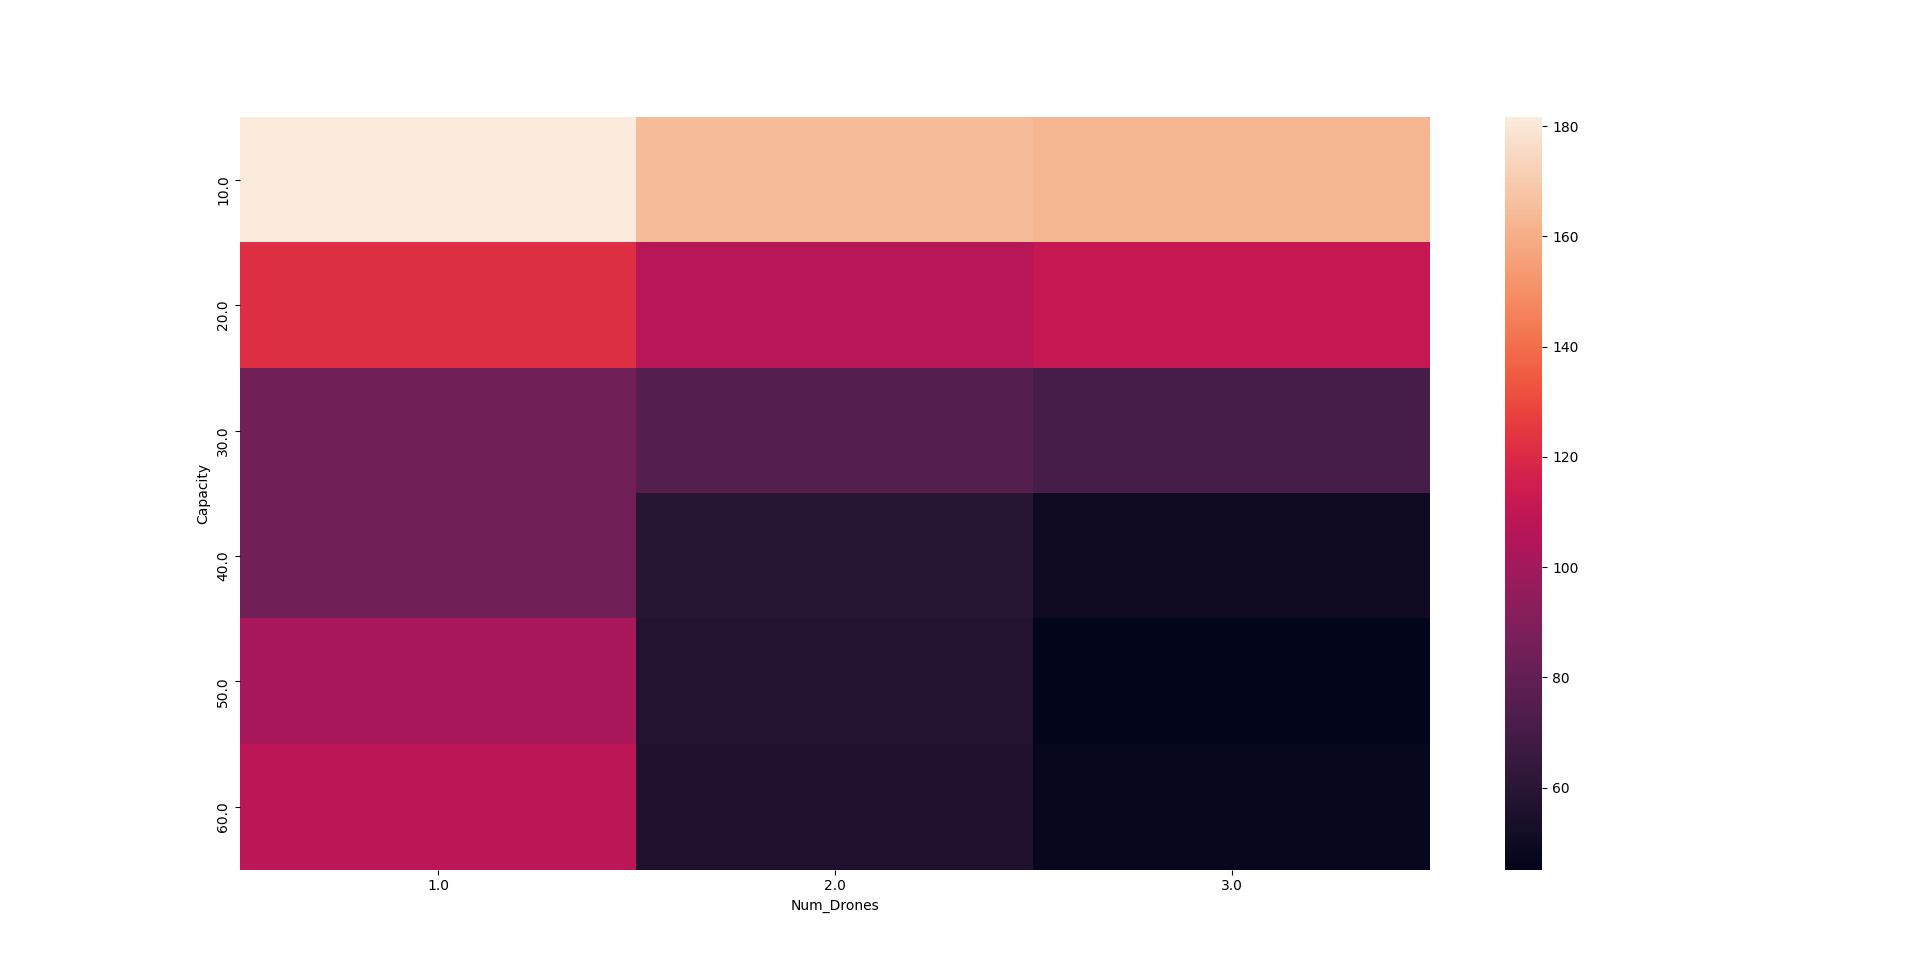
\includegraphics[width=\linewidth]{heatmap.png}
\caption{Heatmap of objective function values depending on number of drones and drone capacities. The darker the color intensity the smaller the objective value. \label{fig:heatmap}}
\end{figure}
\noindent
%In order to test the performances of the matheuristic proposed in Section \ref{Math}, we coded it in Python and we run it on the same sets of instances (Grid and Delaunay) on which the three formulations have been solved. Table \ref{table:tab3} reports for each instance, numbered from 0 to 4, distinguishing between Grid and Delauney, respectively, the best objective function provided by the best formulation, the objective function provided by the matheuristic and the associated CPU time. As already noticed from Table \ref{table:tab2}, for grid graph instances, SEC formulation has the best behaviour, with the exception of the instance number 3 for which the MTZ provides a smaller value of the objective function. As for the Delaunay graph instances, MTZ is the best formulation, but also in this case there is an exception on the instance number 2 for which SEC formulation returns a smaller value of the objective function.\\
%The results show that the matheuristic returns a solution with value of the objective function that is higher than the one provided by the SEC formulation on grid instances. However, these values are smaller than the ones provided by the Stages and the MTZ formulations. Moreover, the saving in terms of resolution time is very significant as the maximum CPU time is less than 1 minute.  As regards the Delaunay instances, the matheuristic performances are even better, as it finds a solution that is better than the best one provided by the MTZ formulation and in a resolution time that is at most 28 minutes. 



%\renewcommand{\arraystretch}{0.7}
%\begin{table}[!h]
%\caption{Heuristic performances}
%\centering
%\footnotesize
%\begin{tabular}{c | c c c | c c c}
%\hline
%\textbf{\#}  & \multicolumn{3}{c}{\textbf{Grid}} &  \multicolumn{3}{c}{\textbf{Delauney}} \\
 % \hline
% &Best Obj & Obj Heuristic &CPU Time &Best Obj & Obj Heuristic & CPU Time \\
%\hline
%0 &	1087,87	& 1117,83 &	50,99 &	947,01 &	934,46 &	52,49\\
%1 &	1100,38	& 1319,64 &	24,64 &	986,22 &	 938,68	& 72,73\\
%2 &	1350,67	& 1126,35 &	46,06 &	888,48 &	865,66 &	1073,80\\
%3 &	1218,66	& 1476,36 &	27,18 &	1249,69 &	1154,62 &	1703,33\\
%4 &	1297,77	& 1424,37 &	40,91 &	1239,93	 & 1184,67 &	81,15\\
%    \hline
%\end{tabular}
%\label{table:tab3}
%\end{table}


\noindent
%We performed a second set of experiments by observing that, even if there are small differences between the SEC and the MTZ formulations depending on the type of instances, their performances are comparable.
%Thus, in the rest of the tests we focused on the MTZ formulation. We compared its performances, with or without providing the initial solution found by the matheuristic, on a set of larger instances. More precisely, we generated 20 instances with targets represented by grid graphs and 20 instances with targets represented by Delauney graphs. The instances of each typology are split in 4 groups of 5 instances each, consisting respectively of 5, 10, 15 and 20 targets to be visited.
%In each instance the same percentage of graphs ($20\%$) has respectively 4, 6, 8, 10 and 12 nodes. 
%Moreover, we assumed that the origin coincides with the destination in all instances and we randomly generated with uniform distribution between 0 and 1, two values representing the percentage of each edge and of each graph to be visited.
%As regards the speeds, we set the speed of the drone three times the one of the mothership.
%We run the MTZ formulation by adopting Gurobi, setting a time limit of 7200 sec. for each instance.
%On the same instances also the matheuristic has been applied. Note that, in order to define a stopping rule for the exact resolution of the AMDRPG model within the matheuristic procedure (STEP 3 and STEP 4), we set the maximum number of solutions generated by the solver equal to five.
%For each instance, the solution provided by the matheuristic has been then used to initialize the exact resolution of the MTZ formulation in order to try to speed up the resolution process.
%Table \ref{table:tab4} shows the results of the comparison between the exact resolution of the formulation with and without initialization. In the first column, named List, we report the size of the instances in terms of number of targets to be visited (0, 1, 2 and 3 identifies instances respectively with 5, 10, 15 and 20 graphs).The second column refers to the two variants of the model, that is, a given percentage of each edge of the targets (e) or a given percentage of each target (g) must be visited by the drone. The other columns report respectively the average percentage gap of the solutions found within the time limit starting from the initial solution provided by the matheuristic, the average running time of the matheuristic and the average percentage gap of the solutions found within the time limit without initialization. These information are reported for both Grid and Delauney instances.

%\renewcommand{\arraystretch}{0.7}
%\begin{table}[!h]
%\caption{Comparison between exact resolution with and without initialization}
%\centering
%\footnotesize
%\begin{tabular}{c c | c c c | c c c}
%\hline
% &  & \multicolumn{3}{c}{\textbf{Grid}} &  \multicolumn{3}{c}{\textbf{Delauney}} \\
%\hline
% List &  $\%$  & $\%$ Gap (i) & Time$\_$h & $\%$ Gap (ni)  & $\%$ Gap (i) & Time$\_$h &  $\%$ Gap (ni)\\
%\hline
%\multirow{}{}{0} & e & 0.72 & 105.12 & 0.73 & 0.78 & 154.92 & 0.74\\
%& g & 0.55 & 58.92 & 0.54 & 0.62 & 92.64 & 0.67\\
%\hline
%\multirow{}{}{1} & e & 0.76 & 241.99 & 0.76 & 0.80 & 314.69 & 0.79\\
%& g & 0.71 & 182.61 & 0.70 & 0.74 & 353.04 & 0.75\\
%\hline
%\multirow{}{}{2} & e & 0.76 & 367.69 & 0.76 & 0.80 & 447.61 & 0.80 \\
%& g & 0.71 & 326.49 & 0.72 & 0.76 & 429.16 & 0.76\\
%\hline
%\multirow{}{}{3} & e & 0.75 & 481.68 & 0.74 & 0.80 & 514.98 & 0.76^*\\
%& g & 0.71 & 492.27 & 0.70 & 0.77 & 582.90 & 0.77\\
%    \hline
%\end{tabular}
%\label{table:tab4}
%\end{table}

\noindent
%From Table \ref{table:tab4} we can notice that in most of the cases the average gaps associated with the solution found within the time limit, with and without initialization by the solution found by the matheuristic, are the same or very close (note that in the last column the $*$ indicates that only one instance has been solved within the time limit).
%As regards the running time of the matheuristic, we can see also from the boxplots in Figure \ref{fig:1}, that it increases with the number of targets to be visited both for Grid and Delaunay instances. Considering the model variants based on the minimum percentage of each edge or each graph to visit, we can observe that for Grid instances the average running time of the model imposing a minimum percentage of each edge to be visited, is greater than the one associated with the other variant, with the exception of the instances of biggest size (List=3). \\
\noindent
%The boxplots in Figure \ref{fig:2} represent the percentage gap of the solution provided by the matheuristic with respect to the one provided by the exact resolution of the MTZ model within the time limit, with initialization by the solution found by the matheuristic. From them we can notice that the gap increases with the size both for Grid and Delaunay instances but it is always less than 0.5$\%$.  
%Figure \ref{fig:3} shows the percentage gap of the solution provided by the exact resolution of the MTZ formulation within the time limit without the initialization, with respect to the one found with the initialization. This gap is very close to 0 both for Grid and Delaunay instances. Only for the biggest size we observe values ranging between 0.1$\%$ and 0.6$\%$. These observations suggest that, even if the initialization of the model by the solution provided by the matheuristic does not speed up the convergence to the optimal solution, the matheuristic provides solutions of very good quality. Indeed, it generates in less than 10 minutes solutions that are very close to the ones provided by the model within 2 hours.\\


%\begin{figure}[htp]% [H] is so declass\'e!
%\centering
%\begin{minipage}{0.45\textwidth}
%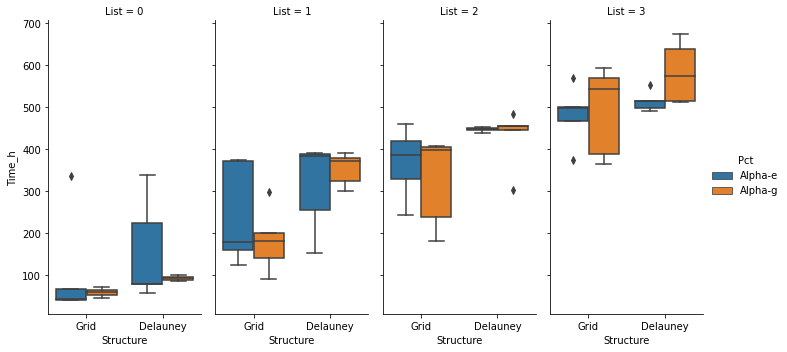
\includegraphics[width=\textwidth]{time_h.png}
%\caption{Matheuristic running time}
%\label{fig:1}
%\end{minipage}\hfill
%\begin{minipage}{0.45\textwidth}
%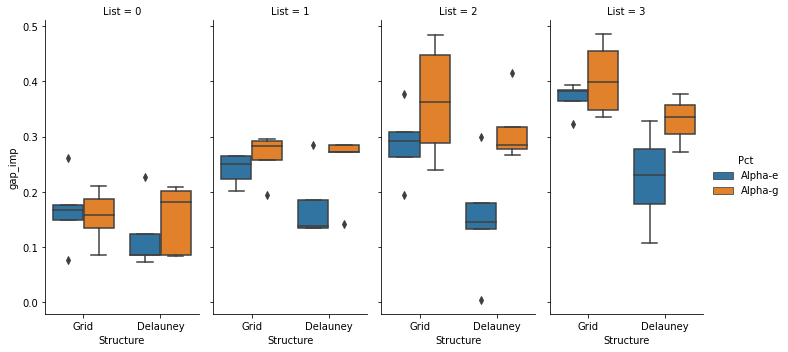
\includegraphics[width=\textwidth]{improved_gap.png}
%\caption{Matheuristic improved gap}
%\label{fig:2}
%\end{minipage}\par
%\vskip\floatsep% normal separation between figures
%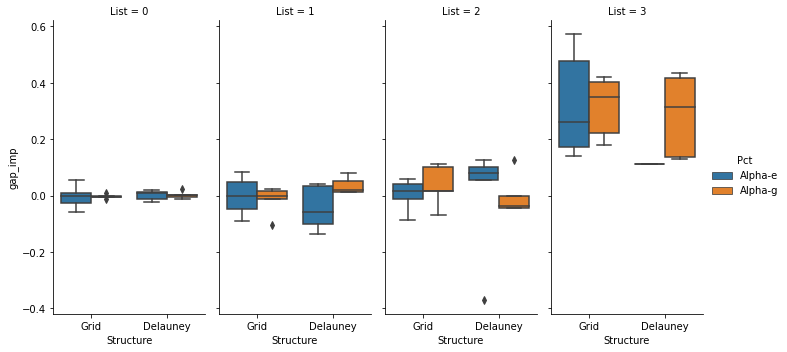
\includegraphics[width=0.45\textwidth]{differencewithwithout.png}
%\caption{Improved gap of MTZ formulation with and without initialization}
%\label{fig:3}
%\end{figure}



%\noindent
%As regards the \NMD \xspace problem, we generated three sets of instances with targets represented by grid graphs considering different structures of the polygonal network where the mothership can move.
%In particular, we defined a first set of instances where the mothership network is represented by a graph of 6 nodes with a tree structure with origin of the path of the base vehicle different from the destination.
%A second set of instances involving a mothership network consisting in a complete graph of 4 vertices with origin of the path of the base vehicle different from the destination.  
%A third set of instances characterized by star graphs of 7 nodes representing the mothership network, where the origin coincides with the destination and it is located at the centre of the star. We generated 10 instances for each of these three classes, 5 of them with 5 targets and 5 with 10 targets to be visited. 
%Moreover, as for the AMDRPG, for each of these 10 instances we randomly generated two values representing the percentage of each edge and of each graph that must be visited by the drone.
%We run on these sets of instances both Stages and MTZ formulations. Table \ref{table:tab5} summarizes the results obtained comparing them. The first column identifies the size of the instances, similarly to Table \ref{table:tab4}, (0 for instances with 5 targets and 1 for instances with 10 targets).
%The second column distinguishes between minimum percentage of each edge (e) or of each graph (g) to be visited by the drone.
%The remaining columns refer to the three different class  of instances described above (1 for the networks with a tree structure, 2 for complete networks and 3 for start networks).
%For each of these sets of instances the average percentage gap of the solutions found within the time limit of 7200 sec. by the two formulations (Stages and MTZ) is reported.


%\renewcommand{\arraystretch}{0.7}
%\begin{table}[!h]
%\caption{Comparison between formulations of \NMD}
%\centering
%\footnotesize
%\begin{tabular}{c c | c c | c c | c c}
%\hline
% & Net Struct  & \multicolumn{2}{c}{1} &  \multicolumn{2}{c}{2}  & \multicolumn{2}{c}{3}\\
%\hline
%List & $\%$ &  Stages  & MTZ & Stages & MTZ  & Stages & MTZ\\
%\hline
%\multirow{}{}{0} & e & 0.89 & 0.33 & 0.88 & 0.24 & 0.87 & 0.39\\
%& g & 0.86 & 0.29 & 0.89 & 0.18 & 0.90 & 0.42\\
%\hline
%\multirow{}{}{1} & e & 0.92 & 0.43 & 0.92 & 0.33 & 0.92 & 0.46\\
%& g & 0.91 & 0.36 & 0.92 & 0.23 & 0.92 & 0.39\\
%\hline
%\end{tabular}
%\label{table:tab5}
%\end{table}

\noindent
%We can observe that for each class of instances and model variants, based on the percentage of each edge or each graph to be visited, the MTZ formulation performs better than the Stages one. In all the cases the percentage average gap associated with the MTZ formulation is one third or half of that associated with the Stages formulation. For this reason, in the following tests, related to the comparison between the exact resolution of the \NMD\xspace  model with and without the initialization by the solution found by the matheuristic, we focused only on the MTZ formulation.\\
%Table \ref{table:tab6} summarizes the results of this comparison distinguishing again between the different network structures (columns labelled 1, 2 and 3), the different size (rows labelled 0 and 1) characterizing the instances and model variants (minimum percentage of each edge (e) or each graph (g) to be visited). For each combination of network structure, size and model variant we reported the average percentage gap with initialization ($\%$ Gap (i)), the solution time of the matheuristic (T$\_$h) and the average percentage gap without initialization by the solution found by the matheuristic ($\%$ Gap (ni))

%\renewcommand{\arraystretch}{0.8}
%\begin{table}[!h]
%\caption{Comparison between exact resolution with and without initialization of \NMD}
%\centering
%\scriptsize
%\begin{tabular}{c c | c c c | c c c | c c c}
%\hline
% & Net Struct  & \multicolumn{3}{c}{1} &  \multicolumn{3}{c}{2}  & \multicolumn{3}{c}{3}\\
%\hline
%List &  $\%$  & $\%$ Gap (i) & T$\_$h & $\%$ Gap (ni)  & $\%$ Gap (i) & T$\_$h &  $\%$ Gap (ni) & $\%$ Gap (i) & T$\_$h &  $\%$ Gap (ni)\\
%\hline
%\multirow{}{}{0} & e & 0.32 & 109.96 & 0.33 & 0.24 & 207 & 0.24 & 0.39 & 177.57 & 0.39\\
%& g & 0.30 & 110.92 & 0.29 & 0.18 & 163.36 & 0.18 & 0.45 & 149.68 & 0.42\\
%\hline
%\multirow{}{}{1} & e & 0.48 & 1030.64 & 0.43 & 0.39 & 802.3 & 0.33 & 0.53 & 770.05 & 0.46\\
%& g & 0.33 & 479.36 & 0.36 & 0.35 & 639.09 & 0.23 & 0.42 & 689.51 & 0.39\\
%\hline
%\end{tabular}
%\label{table:tab6}
%\end{table}

\noindent
%We can observe that, similarly to the AMDRPG problem, the average gaps associated with the solution found within the time limit, with and without initialization by the solution found by the matheuristic, are very close. Considering the average running time we can notice that the \NMD\xspace  problem is more challanging to be solved with respect to the AMDRPG. It increases very fast with the size of the instances especially for the case in which the network where the mothership moves has a tree structure. Moreover, as for the Grid instances in the continuous case, the model variant imposing a minimum percentage of each edge to be visited takes more time to be solved.

%\begin{figure}
%\centering
%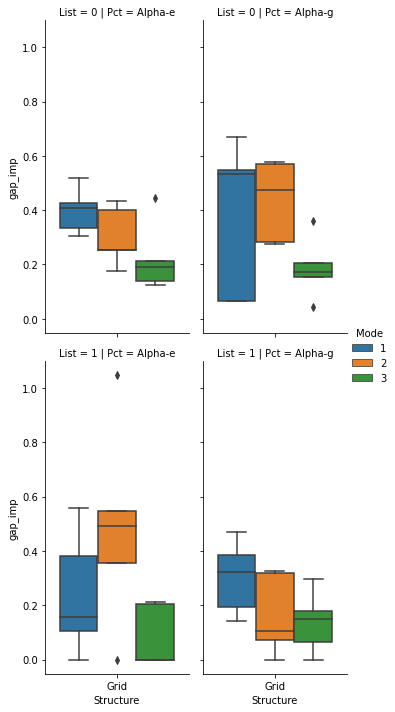
\includegraphics[width=5cm]{improved_gap_ND.png}
%\caption{Matheuristic improved gap for \NMD}
%\label{fig:4}
%\end{figure}
\noindent
%The boxplots showed in Figure \ref{fig:4} report the percentage gap of the solution provided by the matheuristic with respect to the one provided by the exact resolution of the MTZ model within the time limit, with initialization by the solution found by the matheuristic.
%We can notice that, excluding the outliers, this gap ranges between 0$\%$ and 0.7$\%$ and its lowest values are observed for the instances in which the network where the mothership moves has a star structure (green boxplots). 
%From the previous observations, similarly to the AMDRPG, we can conclude that the behaviour of the matheuristic is very good in terms of quality of the solutions provided, even if the initialization of the MTZ model does not help in speeding up the convergence to the optimal solution. 











